\graphicspath{ {./img/capturas} }
\chapter{Introducción}

\section{Presentación}

La elección del lenguaje de programación adecuado es una decisión fundamental en el desarrollo de software. Este proceso implica considerar varios factores, como los requisitos del proyecto, la eficiencia, la facilidad de mantenimiento y la disponibilidad de herramientas y bibliotecas. Una vez seleccionado el lenguaje, surge la necesidad de traducir el código escrito en ese lenguaje a instrucciones que una computadora pueda entender y ejecutar.

La traducción del código se realiza a través de dos enfoques principales: compilación e interpretación. Estos enfoques difieren en su forma de transformar el código fuente en código ejecutable.

\subsection{Compilación}

La compilación implica la traducción del código de alto nivel a código máquina, que es el lenguaje específico de la computadora. Para ilustrar este proceso, consideremos un ejemplo simple en el lenguaje C:

\begin{verbatim}
#include <stdio.h>

int main() {
    printf("Hola, mundo!\n");
    return 0;
}
\end{verbatim}

Cuando compilamos este programa, el compilador traduce el código C a instrucciones específicas del procesador en código máquina. Estas instrucciones se almacenan en un archivo ejecutable, que puede ser ejecutado por la computadora.

\subsection{Interpretación}

En contraste, la interpretación implica ejecutar el código fuente directamente, línea por línea, sin generar un archivo ejecutable independiente. Un ejemplo común de un lenguaje interpretado es Python:

\begin{verbatim}
print("Hola, mundo!")
\end{verbatim}

En este caso, el intérprete de Python ejecuta cada línea de código a medida que se encuentra, generando la salida esperada sin producir un archivo ejecutable.

\subsection{Fases de traducción}

Tanto en la compilación como en la interpretación, el proceso de traducción consta de varias fases:

\begin{enumerate}
    \item \textbf{Análisis}: en esta fase se comprueba que el programa fuente está bien escrito.
    \begin{itemize}
        \item Análisis léxico: divide el código en componentes léxicos (\textit{tokens}) significativos.
        \item Análisis sintáctico: verifica la estructura gramatical del código.
        \item Análisis semántico: examina el significado y la coherencia del código.
    \end{itemize}
    
    \item \textbf{Síntesis}: esta fase se encarga de generar el código del programa ejecutable.
    \begin{itemize}
        \item Generación de código intermedio: crea una representación intermedia del código. Es una fase opcional pero recomendable.
        \item Optimización del código intermedio: permite mejora el código sin tener en cuenta el dispositivo donde se ejecutará. Es una fase opcional pero recomendable.
        \item Generación de código final: produce el código ejecutable o la salida del programa.
        \item Optimización: mejora el código para aumentar su eficiencia.
    \end{itemize}
\end{enumerate}

Estas fases aseguran que el código se traduzca de manera precisa y eficiente, garantizando su funcionamiento correcto.

Además, en el proceso de traducción, juegan un papel fundamental dos componentes auxiliares:

\begin{itemize}
    \item \textbf{Administrador de la tabla de símbolos}: este componente almacena información crucial sobre variables, funciones y otros elementos del programa. Proporciona un registro detallado que permite al traductor acceder y gestionar eficientemente los elementos del código fuente.
    
    \item \textbf{Gestor de errores}: este componente es esencial para manejar cualquier inconveniente que pueda surgir durante la traducción. Detecta y gestiona errores de sintaxis, semántica u otros problemas que podrían comprometer la integridad y funcionalidad del programa final.
\end{itemize}

En la Figura \ref{fig:fases}, se presenta un diagrama que resume las fases principales en el proceso de traducción, desde el análisis hasta la generación del código final.

\begin{figure}[htp]
    \centering
        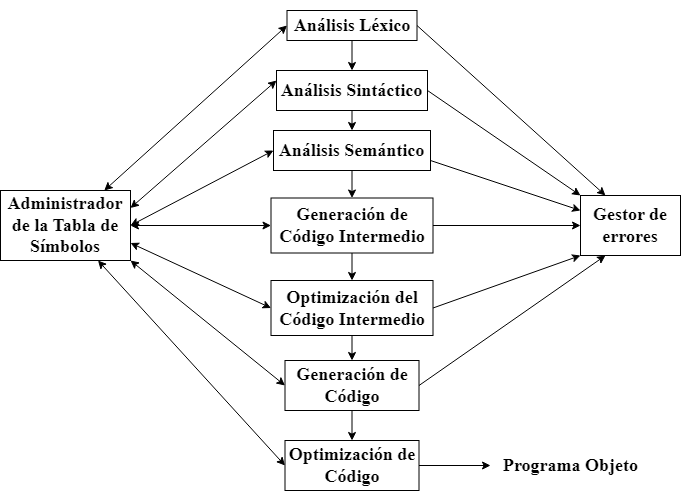
\includegraphics[scale=0.6]{figuras/Cap1/fasescomp.png} \\
    \caption{Fases Principales en el Proceso de Traducción}\label{fig:fases}
\end{figure}

\section{Definición del problema real}

Este proyecto de fin de carrera se enfoca en una tarea crucial: la corrección, mejora y ampliación de ``SimAS: Simuladores de Analizadores Sintácticos'', que es una aplicación desarrollada en java que tiene como objetivo ayudar a la docencia de la asignatura de Procesadores de Lenguajes de tercer curso de la especialidad de Computación del Grado de Ingeniería Informática. 

SimAS proporciona a los estudiantes una comprensión profunda del funcionamiento de la fase de análisis sintáctico en compiladores e intérpretes. Tiene la capacidad de simular tanto analizadores sintácticos descendentes como ascendentes, facilitando que los estudiantes comprendan mejor el funcionamiento de estos métodos de análisis sintáctico.

SimAS es una aplicación de software que posee dos versiones. SimAS 1.0 fue desarrollado por Vanesa González Pérez \cite{vanesa} como Proyecto de Fin de Carrera de Ingeniería Informática en 2015. Esta versión permitía realizar el análisis sintáctico descendente predictivo y el análisis ascendente LR (SLR, LR - canónico y LALR).  Esta versión fue corregida y ampliada en la versión SimAS 2.0, que fue desarrollada por Juan Antonio Fernández Díaz \cite{juan} en su Trabajo de Fin de Grado en 2023. Esta versión permitía generar informes en formato pdf y generar los árboles sintácticos asociados a la derivaciones de los analizadores sintácticos.


A pesar de la funcionalidad satisfactoria de SimAS, se han detectado una serie de errores y deficiencias que demandan atención inmediata.
\begin{itemize}
    \item Al cargar o modificar gramáticas, la aplicación debe ordenar sus reglas de producción en función del símbolo no terminal de la parte izquierda.
    \item Al crear o modificar gramáticas, la aplicación no genera bien el archivo XML \cite{xml} con dicha gramática.
    \item La aplicación no genera o genera de forma incorrecta los informes en formato PDF.
    \item No genera correctamente los conjuntos Primero y Siguiente de algunas gramáticas. Estos conjuntos son necesarios para realizar el análisis sintáctico descendente predictivo y el análisis sintáctico ascendente SLR.
    \item La aplicación no genera correctamente los árboles sintácticos asociados a las derivaciones.
    \item La interfaz produce algunas ventanas no interactivas o que no aportan valor.
\end{itemize}

Además, se pueden incorporar las siguientes mejoras para enriquecer la aplicación:

\begin{itemize}
    \item Diseñar una interfaz más intuitiva que genere todas las ventanas dentro de una misma interfaz y no en diferentes ventanas.
    \item Permitir el trabajo con varias gramáticas a la vez. 
    \item Implementar la posibilidad de cambiar el idioma de la aplicación.
\end{itemize}

Una descripción más detallada de las versiones de SimAS se puede consultar en el capítulo \ref{cap:antecedentes} de Antecedentes.


Aunque las versiones anteriores SimAS 1.0  y 2.0 permiten simular los análisis sintácticos descendente y ascendente, el presente Trabajo de Fin de Grado se va a centrar exclusivamente en corregir todos los fallos encontrados y en mejorar el análisis sintáctico descendente predictivo. La nueva aplicación se denominará ``SimAS 3.0 descendente predictivo''. Se considera que abordar también la corrección de los errores de la simulación del análisis sintáctico ascendente requeriría un esfuerzo superior al exigido en un Trabajo de Fin de Grado. Se debe tener en cuenta que la versión SimAS 2.0 \cite{juan} fue realizada en un Trabajo de Fin de Grado de doble especialidad que tiene una carga docente de 450 horas, superior a las 300 horas de un Trabajo de Fin de Grado de una única especialidad.


\section{Definición del problema técnico}


El presente Trabajo de Fin de Grado pretende desarrollar una aplicación informática multiplataforma, denominada ``SimAS 3.0 descendente predictivo'', que permita corregir y ampliar la simulación del análisis sintáctico descendente predictivo desarrollado en las versiones anteriores de SimAS 1.0 \cite{vanesa} y 2.0 \cite{juan}.

\subsection{Funcionamiento}
La aplicación propuesta se diseñará como una herramienta de escritorio multiplataforma con el objetivo de proporcionar a los usuarios una experiencia interactiva y educativa. Los principales módulos que integrará esta aplicación son los siguientes:

\begin{itemize}
    \item \textbf{Editor de gramáticas de contexto libre:} este módulo permitirá a los usuarios crear, cargar, guardar y modificar gramáticas de contexto libre. La interfaz proporcionará opciones intuitivas para trabajar con las reglas de producción, símbolos terminales y no terminales, así como la definición del símbolo inicial.

    \item \textbf{Simulador gráfico descendente:} esta funcionalidad simulará el proceso de análisis sintáctico descendente predictivo, utilizando la gramática especificada en el editor. El simulador generará una derivación por la izquierda y mostrará el árbol sintáctico descendente resultante.

    \item \textbf{Generación de árboles sintácticos descendentes:} se implementará la funcionalidad para generar árboles sintácticos de forma precisa y visualmente comprensible. Esta característica permitirá a los usuarios visualizar de manera clara la estructura jerárquica de las derivaciones sintácticas.
    
    \item \textbf{Tutorial interactivo:} este módulo proporcionará una guía paso a paso sobre los fundamentos y el funcionamiento de los métodos de análisis sintáctico. Los usuarios podrán acceder a explicaciones detalladas y ejemplos prácticos para comprender mejor los conceptos.
    
    \item \textbf{Ayuda integrada:} se incluirá una sección de ayuda en la interfaz para brindar asistencia instantánea sobre el uso de la aplicación. Los usuarios podrán acceder a información detallada sobre cada componente de la interfaz y los distintos módulos que componen la aplicación.
\end{itemize}

El funcionamiento detallado de cada uno de estos módulos se abordará en el capítulo \ref{cap:especificacion_requisitos} de Especificación de requisitos para proporcionar una comprensión completa de la aplicación.


\subsection{Entorno}
%Posibles modificaciones conforme se desarrolle la aplicación

El entorno en el que se desarrolla y ejecuta una aplicación es fundamental para garantizar su funcionalidad, usabilidad y despliegue efectivo. En este apartado, se detallan los aspectos relacionados con la interfaz de usuario, el entorno de desarrollo y el entorno de ejecución de la aplicación ``SimAS 3.0 descendente predictivo'', proporcionando una visión general de los componentes y requisitos clave para su funcionamiento.


\subsubsection{Interfaz con el usuario}

La aplicación contará con una interfaz gráfica de usuario (GUI\footnote{\textit{Graphical User Interface}}) diseñada para optimizar la experiencia del usuario, especialmente para los estudiantes. Se busca que todo el programa se ejecute en una única ventana, posibilitando la aparición de distintas pestañas, con el fin de simplificar la navegación. 

La interfaz estará diseñada para ser simple y completa al mismo tiempo, permitiendo a los usuarios realizar todas las operaciones necesarias para trabajar con gramáticas. Entre las funcionalidades específicas que ofrecerá la interfaz, se incluyen la capacidad de crear nuevas gramáticas e importar y editar gramáticas creadas previamente. Además, se proporcionará soporte para interacciones complejas, como la entrada de texto y la selección de archivos.

\subsubsection{Entorno de desarrollo}
El desarrollo y mantenimiento del código de la aplicación se realizará utilizando diversas fuentes de información disponibles en Internet, así como técnicas de inteligencia artificial. El entorno de desarrollo integrado (IDE) principal utilizado será IntelliJ \cite{intellij}, que ofrece una amplia gama de características y herramientas para el desarrollo de aplicaciones Java. Además, se utilizarán herramientas adicionales, como sistemas de control de versiones (Git \cite{git}) para el control del código fuente, y se gestionará la documentación y los recursos del proyecto en un repositorio de GitHub \cite{github}.

\subsubsection{Entorno de ejecución}
La aplicación estará diseñada para ser ejecutada en un entorno multiplataforma y compatible con los principales sistemas operativos, incluyendo Windows, macOS y Linux. No se requerirán configuraciones específicas del sistema operativo o del entorno de ejecución para garantizar el funcionamiento correcto de la aplicación. Además, la aplicación se ejecutará en una máquina virtual de Java \cite{java}, lo que proporcionará una mayor portabilidad y compatibilidad con diferentes sistemas. Esto significa que los usuarios finales no necesitarán instalar ninguna dependencia externa ni cumplir con requisitos adicionales de instalación, lo que facilitará su despliegue y uso.


\subsection{Ciclo de mantenimiento} \label{subsec:actualizaciones}

La gestión de actualizaciones de software es un proceso crítico que garantiza la evolución continua y la mejora de la aplicación a lo largo del tiempo. En el caso de ``SimAS 3.0 descendente predictivo'', se implementará un ciclo de mantenimiento diseñado para abordar nuevas funcionalidades, correcciones de errores y adaptaciones a los cambios en los entornos de ejecución.

El ciclo de mantenimiento de ``SimAS 3.0 descendente predictivo'' se basará en un enfoque proactivo y modular, permitiendo la incorporación de mejoras de manera eficiente y sin interrupciones significativas en la experiencia del usuario. Aunque el autor principal del proyecto no asumirá la responsabilidad directa del mantenimiento futuro, se establecerán procedimientos claros para la gestión de actualizaciones, asegurando la continuidad y la calidad del software.

Este enfoque modular no solo facilitará el mantenimiento y la actualización del software, sino que también fomentará la colaboración y la contribución de la comunidad de usuarios y desarrolladores. De esta manera, SimAS 3.0 podrá adaptarse de manera ágil a las necesidades cambiantes de los usuarios y a las demandas del entorno tecnológico.


\subsection{Competencia}

El desarrollo de SimAS 3.0 se sitúa en un contexto de continua evolución y expansión en el ámbito de las herramientas educativas para el análisis sintáctico en la informática. Aunque no buscamos competir comercialmente, es importante comprender el panorama actual y las características distintivas de SimAS 3.0 en relación con otras soluciones disponibles.

A través de un análisis exhaustivo en el Capítulo \ref{cap:antecedentes}, se explorará el terreno de las herramientas educativas existentes para el análisis sintáctico. Se examinarán tanto las aplicaciones desarrolladas en proyectos académicos previos, como otras soluciones disponibles en el mercado. Este análisis permitirá identificar fortalezas, debilidades y oportunidades de mejora para SimAS 3.0.

Si bien se reconocen las contribuciones de otras herramientas educativas, SimAS 3.0 buscará destacarse por su enfoque innovador y sus funcionalidades distintivas. Entre estas funcionalidades, se encuentra la capacidad de generar árboles sintácticos tanto descendentes como ascendentes, ofreciendo una experiencia de aprendizaje única y completa para los estudiantes de informática.


%Posibles modificaciones durante el desarrollo
\subsection{Aspecto externo}

En esta sección, se abordarán aspectos clave relacionados con la experiencia del usuario y la documentación asociada a SimAS 3.0.

\begin{itemize}
    \item \textbf{Diseño de la interfaz de usuario}: la interfaz de usuario de SimAS 3.0 se diseñará cuidadosamente para garantizar una experiencia visual atractiva y una navegación intuitiva. Se prestará especial atención a la disposición de los elementos, la coherencia visual y la accesibilidad, con el objetivo de proporcionar un entorno de trabajo cómodo y eficiente para los usuarios.
    
    \item \textbf{Documentación detallada}:
    \begin{itemize}
        \item \textit{Manual técnico}: este documento proporcionará una descripción exhaustiva de los aspectos técnicos del desarrollo de SimAS 3.0. Se incluirán detalles sobre la arquitectura del software, las tecnologías utilizadas y las decisiones de diseño fundamentales.
        
        \item \textit{Manual de usuario}: el manual de usuario de SimAS 3.0 contendrá instrucciones claras y concisas sobre la instalación, configuración y uso de la aplicación. Se incluirán ejemplos prácticos y capturas de pantalla para guiar al usuario a través de las diferentes funcionalidades de la aplicación.
        
        \item \textit{Manual de código}: este documento estará dirigido a desarrolladores y proporcionará una visión detallada del código fuente de SimAS 3.0. Se describirá la estructura del proyecto, las convenciones de codificación y la documentación interna del código para facilitar su comprensión y mantenimiento.
    \end{itemize}
    
    \item \textbf{Distribución y almacenamiento}: SimAS 3.0 estará disponible para su descarga en línea a través de un repositorio público, lo que facilitará el acceso a la última versión del software y de la documentación asociada. Además, se explorarán opciones para distribuir la aplicación en medios físicos o mediante servicios de almacenamiento en la nube, asegurando así su disponibilidad y accesibilidad para los usuarios.
\end{itemize}


\subsection{Estandarización}

En esta sección, se describirán los principios de diseño y usabilidad que guiarán el desarrollo de SimAS 3.0, con el objetivo de garantizar una experiencia de usuario coherente y satisfactoria.

\begin{itemize}
    \item \textbf{Diseño centrado en el usuario}: SimAS 3.0 se diseñará pensando en las necesidades y expectativas del usuario final. Se realizarán investigaciones de usuarios y pruebas de usabilidad para asegurar que la interfaz de usuario sea intuitiva y fácil de usar.
    
    \item \textbf{Consistencia y coherencia}: la interfaz de usuario de SimAS 3.0 mantendrá una apariencia y comportamiento coherentes en todas sus funciones y elementos. Se seguirán estándares de diseño reconocidos y se aplicarán patrones de diseño comunes para garantizar una experiencia consistente para el usuario.
    
    \item \textbf{Sensibilidad y guía del usuario}: la interfaz de SimAS 3.0 guiará al usuario a través de la aplicación, proporcionando retroalimentación clara y orientación en cada paso del proceso. Se utilizarán mensajes informativos y visuales para informar al usuario sobre el estado y las acciones disponibles.
    
    \item \textbf{Interacción intuitiva}: se priorizará una interacción sencilla y fluida en SimAS 3.0. Los controles y las funciones de la aplicación se diseñarán de manera intuitiva, minimizando la necesidad de aprendizaje por parte del usuario y facilitando el uso de la aplicación desde el primer momento.
    
    \item \textbf{Claridad y legibilidad}: la interfaz gráfica de SimAS 3.0 se diseñará con un enfoque en la claridad y la legibilidad. Se utilizarán colores y tipografías adecuados para garantizar una fácil comprensión de la información presentada, evitando la sobrecarga visual y la confusión del usuario.
\end{itemize}


\subsection{Calidad y fiabilidad}

En esta sección, se abordarán los aspectos de calidad, fiabilidad y seguridad que son fundamentales en el desarrollo y uso de SimAS 3.0. Se buscará garantizar el correcto funcionamiento de la aplicación, así como proteger la integridad y privacidad de los usuarios.

\begin{itemize}
    \item \textbf{Calidad y fiabilidad}: SimAS 3.0 se desarrollará con un enfoque en la calidad del software y la fiabilidad de su funcionamiento. Se utilizarán herramientas actualizadas como IntelliJ IDEA y la Máquina Virtual de Java para respaldar la calidad del código y su ejecución. Además, la aplicación será sometida a exhaustivas pruebas para detectar y corregir errores antes de su lanzamiento.
    
    \item \textbf{Seguridad}: la seguridad de SimAS 3.0 será una prioridad, tanto en términos de protección contra acciones incorrectas por parte del usuario como en la seguridad del dispositivo de almacenamiento. Se implementarán mecanismos de seguridad en la aplicación para evitar cualquier manipulación maliciosa o acceso no autorizado a los datos del usuario. Se garantizará que el usuario no tenga acceso a ninguna funcionalidad aparte de aquellas proporcionadas explícitamente por la aplicación, asegurando así que no se realicen acciones no deseadas ni se acceda a datos sensibles. Asimismo, se garantizará que la distribución y uso de la aplicación cumplan con los principios de software libre, siguiendo la licencia GPL de GNU para proteger su distribución y uso adecuados.
\end{itemize}


\subsection{Validación y verificación}

El proceso de validación y verificación de SimAS 3.0 es esencial para garantizar su correcto funcionamiento y la detección temprana de posibles errores.

\begin{itemize}
    \item \textbf{Validación}: se centrará en asegurar que la aplicación cumple con los requisitos y expectativas del usuario final. Se llevarán a cabo pruebas funcionales para verificar que todas las funcionalidades operan según lo esperado, y se realizarán pruebas de aceptación para garantizar que la aplicación satisface las necesidades del usuario.
    
    \item \textbf{Verificación}: por otro lado, se centrará en asegurar que el código y la lógica de la aplicación son correctos y libres de errores. Se realizarán pruebas unitarias para verificar el correcto funcionamiento de cada componente individualmente, así como pruebas de integración para garantizar que los componentes interactúan correctamente entre sí.
\end{itemize}

El proceso estará dividido en varias etapas, cada una con su respectiva documentación detallada:

\begin{itemize}
    \item \textbf{Planificación de pruebas}: se definirán los objetivos y alcance de las pruebas, así como los recursos y herramientas necesarios para llevarlas a cabo.
    
    \item \textbf{Diseño de pruebas}: se elaborará un plan detallado de las pruebas a realizar, incluyendo los casos de prueba específicos y los criterios de aceptación.
    
    \item \textbf{Ejecución de pruebas}: se llevarán a cabo las pruebas según el plan establecido, registrando los resultados obtenidos y cualquier incidencia detectada.
    
    \item \textbf{Análisis de resultados}: se analizarán los resultados de las pruebas para identificar posibles áreas de mejora o corrección. Se documentarán los errores encontrados y se propondrán soluciones para su resolución.
\end{itemize}

El capítulo \ref{cap:pruebas} detallará cada una de estas etapas y proporcionará una visión completa del proceso de validación y verificación de SimAS 3.0.


\subsection{Programa de tareas}

El desarrollo del Trabajo de Fin de Grado estará compuesto por las siguientes actividades:
\begin{enumerate}
    \item \textbf{Exploración inicial} 
        \begin{itemize}
            \item Comprensión y prueba de SimAS 2.0 \cite{juan}.
            \item Definición del problema técnico.
            \item Establecimiento de los objetivos.
            \item Revisión de los antecedentes.
            \item Identificación de los recursos iniciales y estratégicos.
            \item Selección de las herramientas de software y hardware.
            \item Investigación del entorno Intellij \cite{intellij} y del lenguaje de programación Java \cite{java}.
        \end{itemize}
    \item \textbf{Análisis y diseño}
        \begin{itemize}
            \item Especificación de requisitos: funcionales, no funcionales, de información y de la interfaz.
            \item Elaboración de los casos de uso.
            \item Validación de los casos de uso.
            \item Elaboración de los diagramas de secuencia.
        \end{itemize}
    \item \textbf{Diseño}
        \begin{itemize}
            \item Diseño de la arquitectura del sistema.
            \item Diseño de paquetes y clases.
            \item Diseño de la interfaz
        \end{itemize}        
    \item \textbf{Implementación}
        \begin{itemize}
            \item Desarrollo del código.
            \item Implementación de pruebas unitarias.
            \item Validación del código desarrollado.
        \end{itemize} 
    \item \textbf{Documentación}
      \begin{itemize}
          \item Elaboración del manual técnico, manual de usuario y manual de código.
          \item La redacción del manual técnico se realizará durante todo el proceso de desarrollo del Trabajo de Fin de Grado.
      \end{itemize}
\end{enumerate}

\subsection{Pruebas}
Las pruebas y la validación son elementos esenciales en el desarrollo de cualquier aplicación. Estos procesos permiten asegurar que la aplicación cumpla con los estándares de calidad y funcionalidad esperados. En el caso de SimAS 3.0, se llevarán a cabo diversas actividades de evaluación y validación para garantizar su correcto funcionamiento y fiabilidad.

\subsubsection{Tipos de Pruebas}

Se llevarán a cabo varios tipos de pruebas para evaluar distintos aspectos de SimAS 3.0:

\begin{itemize}
    \item \textbf{Pruebas de Funcionalidad:} estas pruebas se centran en verificar que todas las funciones y características de SimAS 3.0 funcionen como se espera. Se realizarán pruebas exhaustivas para cada módulo y componente de la aplicación.
    
    \item \textbf{Pruebas de Interfaz de Usuario:} estas pruebas se enfocarán en la usabilidad y la experiencia del usuario. Se evaluará la interfaz gráfica para garantizar que sea intuitiva y fácil de usar.

    \item \textbf{Pruebas de Rendimiento:} se llevarán a cabo pruebas para evaluar el rendimiento y la velocidad de SimAS 3.0, especialmente en situaciones de carga y con grandes conjuntos de datos.

    \item \textbf{Pruebas de Compatibilidad:} se realizarán pruebas en diferentes sistemas operativos y entornos de ejecución para garantizar que SimAS 3.0 funcione correctamente en diversas configuraciones.
\end{itemize}

\subsubsection{Descripción de las Pruebas}

Cada prueba estará estructurada de la siguiente manera:

\begin{itemize}
    \item \textbf{Objetivo:} se definirá claramente el objetivo de la prueba, es decir, qué se espera evaluar o validar.
    
    \item \textbf{Problema:} se identificarán y documentarán los problemas o errores detectados durante la ejecución de la prueba, junto con información detallada sobre cómo reproducirlos.

    \item \textbf{Solución:} se propondrán soluciones y acciones correctivas para abordar los problemas identificados durante las pruebas, asegurando así la mejora continua de la aplicación.
\end{itemize}

El próximo capítulo \ref{cap:pruebas} detallará los procedimientos y resultados de las pruebas llevadas a cabo en ``SimAS 3.0 descendente predictivo'' como parte de este Trabajo de Fin de Grado.


\subsection{Seguridad}
La seguridad en la presente aplicación se centra principalmente en garantizar su correcto funcionamiento sin comprometer la integridad de los sistemas donde se ejecute. Dado que la aplicación no maneja ni almacena datos personales de los usuarios, el enfoque de seguridad se orienta hacia la prevención de posibles daños a los equipos o entornos de ejecución.

Se implementarán medidas para asegurar que durante la ejecución de la aplicación, los usuarios no puedan realizar acciones que puedan comprometer su funcionamiento o la estabilidad del sistema. Además, se prestará especial atención a la protección del dispositivo de almacenamiento donde se ejecute la aplicación, garantizando que no se produzcan daños o alteraciones no deseadas.

En línea con la versión anterior, la aplicación se distribuirá libremente, sin restricciones de uso, copia o distribución. Esto se fundamenta en su naturaleza académica y en su carácter no lucrativo. No se aplicarán medidas de protección contra la distribución libre de la aplicación, permitiendo su acceso y uso por parte de cualquier usuario interesado en aprender o utilizarla con fines educativos.

En cuanto a la licencia, la aplicación seguirá los principios de la Licencia Pública General de GNU (GPL), que garantiza la libertad de uso, modificación y redistribución del software. Esta licencia ayuda a prevenir acciones malintencionadas relacionadas con la copia o reproducción del software, asegurando que permanezca accesible para la comunidad académica y de desarrollo de software.